\section{Finite-time examples and numerical comparisons on Sol}

\subsection{Initial data and checks for finite blocks}

For Sol Gowdy take $n=1$ and initialize at $t=1$ from $p=J_0(kt)$ and $r=J_0(\sqrt{k^2+4}\,t)/2$ and their derivatives. For Nil base modes use wavevector $(1,0)$, $P=\sqrt2p\cos x$, $Q=\sqrt2q\sin x$ and $(p,p_u,q,q_u)=(0.2,0.07,-0.1,0.03)$ at $u=1$. Initial Hamiltonian momenta are obtained from (N-01).

For central Nil take $m=1,r=0,L=2$, with $Q=0$, $\Pi=(0.03,-0.02)$ at $u=1$. For $S^3$, excite left $m=+3/2$ at $j=3/2$ with $Q=0$, first momentum $0.03$ and sixth momentum $-0.02$ among the eight entries, at $\tau=1/4$, and add its real-field conjugate at left $m=-3/2$. Other entries initially vanish; all right indices and reconstructed metric components are retained.

DOP853 runs compare relative tolerances $10^{-10}$ and $10^{-12}$, with absolute tolerance smaller by a factor of 100, at 201 times on each interval. The table reports maximum component differences for the finer run, not rigorous error bounds.

\begin{center}\small\begin{tabularx}{\textwidth}{@{}>{\raggedright\arraybackslash}X>{\raggedright\arraybackslash}X>{\raggedright\arraybackslash}X>{\raggedright\arraybackslash}X@{}}\toprule
Example & Independent comparison & Maximum difference & Constraint\\\midrule
Nil base & Second order / Hamilton & $1.13\times10^{-12}$ & $3.89\times10^{-16}$\\
Nil central & Reduced / full ADM & $7.30\times10^{-13}$ & $6.94\times10^{-17}$\\
Sol Gowdy & Numerical / Bessel & $2.61\times10^{-12}$ & Analytic reconstruction\\
$S^3$ Taub & Reduced / full ADM & $1.45\times10^{-13}$ & $2.22\times10^{-15}$\\
\bottomrule\end{tabularx}\end{center}

The central Nil charge and all four $S^3$ charges vanish for these initial data and remain zero to numerical precision. These comparisons support finite-time linear examples. These numerical comparisons do not construct an exact nonlinear family. Local integrability of the admissible Sol initial data follows independently from the theorem application (SL-01).

\subsection{Independent four-dimensional Lorenz system on Sol}

\stepcounter{equation}\begin{equation}\tag{SH-01}\label{eq:SH-01}
\begin{aligned}
\mathcal F_\nu&=\nabla^\mu h_{\mu\nu}-\tfrac12\nabla_\nu h^\mu{}_\mu,\\
\delta R_{\mu\nu}-\nabla_{(\mu}\mathcal F_{\nu)}&=0,\qquad
H_{tt}=H_{\xi\xi}+B_xH_\xi+B_tH_t+B_0H.
\end{aligned}
\end{equation}

Direct Ricci variation in the noncoordinate frame of $\mathrm{diag}(-F,F,t,t)$ gives (SH-01). We use the standard Lorenz hyperbolic reduction, without WKB or geometric-optics approximations \cite{Andersson2021}. The ten components are ordered $(00,01,02,03,11,22,33,12,13,23)$ with phases $(1,1,i,i,1,1,1,i,i,1)$ to make coefficients real.

\stepcounter{equation}\begin{equation}\tag{SH-02}\label{eq:SH-02}
\begin{aligned}
H_{00}(1)=H_{0i}(1)&=0,\quad (h,p)(1)=E(1)y(1),\\
\mathcal F(1)&=\dot{\mathcal F}(1)=0,\qquad
y=-J_rE^\dagger Jz,\quad (-J_rE^\dagger J)E=I,\\
(-J_rE^\dagger J)JC^\dagger&=0.
\end{aligned}
\end{equation}

Match the spatial $H,\dot H$ to the same constrained ADM initial data, and determine $\dot H_{00},\dot H_{0i}$ from the Lorenz condition. The independent wave equation and ADM constraints also give $\dot{\mathcal F}(1)=0$ exactly. The projection (SH-02) removes gauge directions before comparison with the reduced variables $y$ of Appendix G; raw metric components in different gauges are not equated. All $B$ matrices and initial maps are supplied in the public supplement, implementing (RG-01) and direct Ricci variation.

\stepcounter{equation}\begin{equation}\tag{SH-03}\label{eq:SH-03}
\begin{aligned}
(n_1,n_2)&=(1,0),\quad \xi_0=\tfrac12\log(k_0/l_0),\\
y_\alpha(1,\xi)&=8^{1/4}\sum_{n=0}^{31}c_{\alpha n}
 \psi_n(\sqrt8(\xi-\xi_0)),\qquad \alpha=1,\ldots,4.
\end{aligned}
\end{equation}

The 128 coefficients are fixed in \texttt{data/initial/sol\_profile.json}, with a checked hash. They define the common initial profile. The profile is fixed input and is not interpreted as a conserved physical mode or frequency. Here $\psi_n$ is the normalized Hermite function; neither the orbit nor the basis is changed with time.

\subsection{Fixed discretization and three convergence comparisons}

\stepcounter{equation}\begin{equation}\tag{SH-04}\label{eq:SH-04}
\xi_j=\xi_0-W+\frac{2Wj}{N+1},\quad j=1,\ldots,N,\qquad
H(t,\xi)=\sum_{n=1}^N a_n(t)\sin\frac{n\pi(\xi-\xi_0+W)}{2W}.
\end{equation}

Use the time-fixed sine basis (SH-04), homogeneous Dirichlet conditions at its endpoints and DST spatial derivatives. These boundary conditions do not guarantee constraint preservation. On $|\xi-\xi_0|\le4$, $1\le t\le2$, continuum characteristic speed one leaves a margin of $0.25$ for $W=5.25$. The nonlocal spectral truncation is separately checked by changing the window; continuum causality alone does not imply zero numerical boundary error.

\begin{center}\small\begin{tabularx}{\textwidth}{@{}>{\raggedright\arraybackslash}X>{\raggedright\arraybackslash}X>{\raggedright\arraybackslash}X@{}}\toprule
Comparison & Parameters & Maximum reduced $L^2$ difference\\\midrule
Space &  $N=1023\to1535$, $W=5.25$ & $3.2645\times10^{-8}$\\
Window & $W=5.25\to5.6875$, $N=1535\to1663$ & $2.7682\times10^{-10}$\\
Time & rtol $10^{-12}\to3\times10^{-14}$, $N=1535$ & $3.9359\times10^{-9}$\\
\bottomrule\end{tabularx}\end{center}

Spatial and window comparisons use relative tolerance $3\times10^{-14}$ and absolute tolerance $3\times10^{-16}$. The window comparison keeps the grid spacing fixed. Fields at 101 saved times are interpolated to the same 2048-point interior Gauss--Legendre quadrature. The relative tolerance approaches double precision; the table reports numerical comparisons for this implementation.

\begin{figure}[htbp]\centering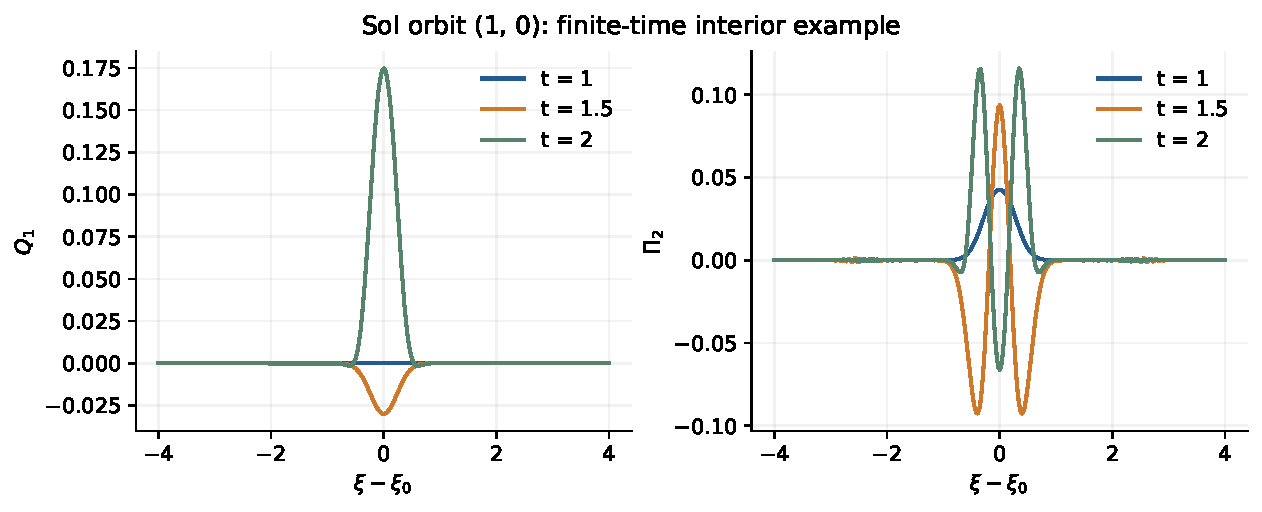
\includegraphics[width=.92\textwidth]{figures/fig05_sol_interior.pdf}
\caption{Reconstructed $Q_1$ and $\Pi_2$ on the interior from the same Sol initial profile. These are reduced variables in a finite-time example, not a gauge-independent metric observation or physical spectrum.}\label{fig:fig05_sol_interior}
\end{figure}

\subsection{Continuous-time residuals and unresolved scope}

\stepcounter{equation}\begin{equation}\tag{SH-05}\label{eq:SH-05}
\|v\|_I=\left(\int_{\xi_0-4}^{\xi_0+4}\sum_a|v_a|^2d\xi\right)^{1/2},\qquad
\rho_{\rm red}=\frac{\|\dot y-J_rH_ry\|_I}{\max(1,\|J_rH_ry\|_I)}.
\end{equation}

Analytically differentiate the actual accepted seventh-degree DOP853 dense polynomial at twenty times $t=1.025+0.05j$, $j=0,\ldots,19$, to obtain $H,\dot H,\ddot H$. These derivatives are substituted directly into the independent Ricci operator and the reduced fourth-order system (SG-05); $\ddot H$ is not replaced by the wave equation in (SH-01). Polynomial values are also compared directly with SciPy interpolation.

\begin{center}\small\begin{tabularx}{\textwidth}{@{}>{\raggedright\arraybackslash}X>{\raggedright\arraybackslash}X@{}}\toprule
Diagnostic & Maximum on the interior\\\midrule
Lorenz wave equation & $5.8631\times10^{-10}$\\
All ten Einstein components & $3.8255\times10^{-11}$\\
Lorenz constraint & $9.4853\times10^{-15}$\\
ADM constraint & $2.4617\times10^{-12}$\\
Reduced fourth-order $\rho_{\rm red}$ & $1.5388\times10^{-3}$\\
\bottomrule\end{tabularx}\end{center}

The first four rows are unnormalized $L^2$ norms of fixed-frame components; the last is the normalized residual (SH-05) of the reduced fourth-order system. Their magnitudes are not directly comparable error criteria. At the twenty times $\|J_rH_ry\|_I$ lies between $0.13$ and $2.7$, so the denominator in (SH-05) switches between absolute and relative normalization. The same residual is also evaluated on the four trajectories of the convergence comparisons at the 21 saved times $t=1,1.05,\ldots,2$, with $\ddot H$ given by the wave equation in (SH-01).

\begin{center}\small\begin{tabularx}{\textwidth}{@{}>{\raggedright\arraybackslash}X>{\raggedright\arraybackslash}X@{}}\toprule
Trajectory & Maximum $\rho_{\rm red}$ at the saved times\\\midrule
$N=1023$, $W=5.25$, rtol $3\times10^{-14}$ & $9.7624\times10^{-4}$\\
$N=1535$, $W=5.25$, rtol $3\times10^{-14}$ & $1.3726\times10^{-3}$\\
$N=1663$, $W=5.6875$, rtol $3\times10^{-14}$ & $9.6257\times10^{-4}$\\
$N=1535$, $W=5.25$, rtol $10^{-12}$ & $4.5461\times10^{-3}$\\
\bottomrule\end{tabularx}\end{center}

From $N=1023$ to $N=1535$ the residual does not decrease, and with the looser time tolerance it grows by a factor of about three. Convergence in the reduced fourth-order form is therefore not established. The independent Lorenz comparison supports a finite-time interior example. Whole-line error bounds, all-orbit or all-time stability and physical spectra remain unestablished. The continuous initial profile (SH-03) is covered by (SL-01), which does not certify exactness or convergence of the finite-window numerical trajectory.
